\documentclass[11pt,a4paper]{article}

% ── Packages ──────────────────────────────────────────────────────────────────
\usepackage[T1]{fontenc}
\usepackage[utf8]{inputenc}
\usepackage[margin=2.2cm]{geometry}
\usepackage{lmodern}
\usepackage{microtype}
\usepackage{xcolor}
\usepackage{booktabs}
\usepackage{tabularx}
\usepackage{amsmath}
\usepackage{listings}
\usepackage{hyperref}
\usepackage{fancyhdr}
\usepackage{titlesec}
\usepackage{enumitem}
\usepackage{tcolorbox}
\usepackage{tikz}
\usetikzlibrary{shapes.geometric, arrows.meta, positioning, calc, backgrounds}

% ── Colours ───────────────────────────────────────────────────────────────────
\definecolor{Blue}  {HTML}{1F6FEB}
\definecolor{Green} {HTML}{2DA44E}
\definecolor{Orange}{HTML}{E36209}
\definecolor{Purple}{HTML}{8250DF}
\definecolor{Gold}  {HTML}{BF8700}
\definecolor{Gray}  {HTML}{57606A}
\definecolor{Light} {HTML}{F6F8FA}
\definecolor{Red}   {HTML}{CF222E}

% ── Code style ────────────────────────────────────────────────────────────────
\lstset{
  basicstyle=\ttfamily\small,
  keywordstyle=\color{Blue}\bfseries,
  commentstyle=\color{Gray}\itshape,
  stringstyle=\color{Green},
  backgroundcolor=\color{Light},
  frame=single, rulecolor=\color{Gray!30},
  numbers=left, numberstyle=\tiny\color{Gray},
  breaklines=true, captionpos=b
}

% ── Coloured boxes ────────────────────────────────────────────────────────────
\tcbuselibrary{skins,breakable}
\newtcolorbox{idea}[1]{colback=Blue!6,colframe=Blue,
  title=\textbf{#1},fonttitle=\sffamily,breakable}
\newtcolorbox{note}[1]{colback=Orange!6,colframe=Orange,
  title=\textbf{#1},fonttitle=\sffamily,breakable}
\newtcolorbox{tip}[1]{colback=Green!6,colframe=Green,
  title=\textbf{#1},fonttitle=\sffamily,breakable}

% ── Page style ────────────────────────────────────────────────────────────────
\pagestyle{fancy}\fancyhf{}
\fancyhead[L]{\textcolor{Blue}{\textbf{Spectrum-SLM}} \ Technical Reference}
\fancyhead[R]{\textcolor{Gray}{\small SDR Cognitive Radio · April 2026}}
\fancyfoot[C]{\thepage}
\renewcommand{\headrulewidth}{0.5pt}

% ── Section formatting ────────────────────────────────────────────────────────
\titleformat{\section}  {\color{Blue}\Large\bfseries\sffamily} {}{0pt}{}[\color{Blue}\hrule\vspace{2pt}]
\titleformat{\subsection}{\color{Blue!70!black}\large\bfseries\sffamily}{}{0pt}{}
\titleformat{\subsubsection}{\color{Gray}\normalsize\bfseries\sffamily}{}{0pt}{}

% ── TikZ common styles ────────────────────────────────────────────────────────
\tikzset{
  blk/.style={draw, rounded corners=5pt, align=center, font=\small\sffamily,
              minimum height=0.85cm, minimum width=3.2cm},
  arr/.style={-Stealth, thick}
}

\hypersetup{colorlinks,linkcolor=Blue,urlcolor=Blue}

% =============================================================================
\begin{document}
% =============================================================================

% ── Title block ───────────────────────────────────────────────────────────────
\begin{center}
  {\color{Blue}\rule{\textwidth}{2pt}}\\[6pt]
  {\Huge\bfseries\sffamily Spectrum-SLM}\\[4pt]
  {\large\sffamily\color{Gray} Technical Reference — PTH Files · Transformer Architecture · Flowcharts}\\[6pt]
  {\small\sffamily Anjani \textbullet{} Ashish Joshi \textbullet{} Mayank \quad|\quad
   Guide: Dr.~Abhinandan S.P. \quad|\quad April 2026}\\[6pt]
  {\color{Blue}\rule{\textwidth}{1pt}}
\end{center}

\tableofcontents
\vspace{1em}

% =============================================================================
\section{What is Spectrum-SLM?}
% =============================================================================

\begin{idea}{One-Line Summary}
Spectrum-SLM is a \textbf{Small Language Model (SLM)} that ``reads'' a radio
spectrum snapshot (a 176-number PSD vector from an SDR) and tells you:
\textbf{(1)} Is the channel busy?  \textbf{(2)} What modulation is in use?
\textbf{(3)} What is the SNR?
\end{idea}

\noindent It trains in \textbf{three phases}, each building on the last:

\begin{center}
\begin{tabular}{clll}
\toprule
\textbf{Phase} & \textbf{Name} & \textbf{Analogy} & \textbf{What it learns} \\
\midrule
1 & Masked Spectrum Modelling & BERT pre-training   & Spectrum structure, without labels \\
2 & Supervised Fine-Tuning    & BERT fine-tuning     & PU detection, modulation, SNR \\
3 & Generative Modelling      & GPT next-token pred. & Predict the next PSD snapshot \\
\bottomrule
\end{tabular}
\end{center}

% =============================================================================
\section{PTH / PT File Reference}
% =============================================================================

\begin{idea}{Two kinds of \texttt{.pth/.pt} files}
\begin{itemize}[nosep]
  \item \textbf{Dataset \texttt{.pth}} — Python dicts of raw PSD captures
        from GNURadio/USRP. One file per modulation scheme, stored inside
        \texttt{Secondary\_User/}.
  \item \textbf{Checkpoint \texttt{.pt}} — PyTorch model weights snapshot
        saved after each training phase. Stored inside
        \texttt{checkpoints/} and \texttt{slm\_checkpoints/}.
\end{itemize}
\end{idea}

% ─────────────────────────────────────────────────────────────────────────────
\subsection{Dataset Files — \texttt{Secondary\_User/}}
% ─────────────────────────────────────────────────────────────────────────────

\subsubsection{File List and Purpose}

\begin{table}[h!]
\centering
\caption{All dataset \texttt{.pth} files — location, modulation, format type and size}
\renewcommand{\arraystretch}{1.4}
\begin{tabularx}{\textwidth}{>{\ttfamily\footnotesize}l l l X r}
\toprule
\textbf{File name} & \textbf{Modulation} & \textbf{Format} & \textbf{Description} & \textbf{Size}\\
\midrule

psd\_binned\_by\_snr\_.pth
  & Mixed / unknown & Binned
  & Captures without a fixed modulation. Useful for Phase 1
    self-supervised pre-training where labels are not required.
  & 41 MB \\[4pt]

psd\_binned\_by\_snr\_bpsk.pth
  & BPSK & Binned
  & Largest single-modulation file. BPSK produces a narrow,
    high-peaked single-lobe PSD. Covers 9 SNR bins (4–20\,dB).
    Each sample = (176-bin PSD vector, PU label 0/1).
  & 90 MB \\[4pt]

psd\_binned\_by\_snr\_qpsk.pth
  & QPSK & Binned
  & QPSK spectrum is slightly wider than BPSK (2 bits/symbol).
    Same 9 SNR bins. Same per-sample format as BPSK file.
  & 63 MB \\[4pt]

psd\_binned\_by\_snr\_16qam.pth
  & 16-QAM & Binned
  & 16 amplitude/phase levels; broadest PSD of the binned set
    (4 bits/symbol). Wider bandwidth visible in PSD shape.
  & 53 MB \\[4pt]

psd\_log\_16qam.pth
  & 16-QAM & Log-scale
  & Lighter format — PSDs stored \emph{directly in dB},
    no SNR binning. Used as a secondary / cross-validation source.
  & 21 MB \\[4pt]

psd\_log\_8psk.pth
  & 8-PSK & Log-scale
  & Same lighter log-scale format as above, for 8-PSK modulation
    (3 bits/symbol). 8-PSK sits spectrally between QPSK and 16-QAM.
  & 20 MB \\
\bottomrule
\end{tabularx}
\end{table}

\subsubsection{Binned Format — Internal Object Layout}

Every \texttt{psd\_binned\_by\_snr\_*.pth} is a Python \texttt{dict}
with exactly \textbf{two keys}:

\begin{center}
\renewcommand{\arraystretch}{1.35}
\begin{tabularx}{\textwidth}{>{\ttfamily}l l X}
\toprule
\textbf{Key} & \textbf{Python type} & \textbf{What it contains} \\
\midrule
\texttt{bins}
  & \texttt{list[float]}
  & The 9 SNR bin centre values in dB:
    \texttt{[4.0, 6.0, 8.0, 10.0, 12.0, 14.0, 16.0, 18.0, 20.0]}.
    These are the only SNR levels captured. \\[4pt]
\texttt{pairs\_by\_bin}
  & \texttt{dict[float $\to$ list[tuple]]}
  & Maps each bin value to a \textbf{list of (psd\_vector, pu\_label) pairs}.
    The list length varies by modulation and SNR (typically thousands per bin).\\
\bottomrule
\end{tabularx}
\end{center}

\smallskip
\noindent Each \textbf{tuple} inside the list contains:

\begin{center}
\renewcommand{\arraystretch}{1.35}
\begin{tabularx}{\textwidth}{>{\ttfamily}l l l X}
\toprule
\textbf{Element} & \textbf{Type} & \textbf{Shape} & \textbf{Description} \\
\midrule
psd\_vector
  & \texttt{numpy.ndarray} or \texttt{list}
  & \texttt{(176,)} \texttt{float32}
  & The full Power Spectral Density vector in dB. 176 frequency bins
    spanning the USRP sample bandwidth. Captured via Welch's method
    in GNURadio with a fixed FFT size. \\[4pt]
pu\_label
  & \texttt{int}
  & scalar
  & Ground-truth Primary User occupancy:
    \textbf{0} = channel idle (PU absent),
    \textbf{1} = channel occupied (PU transmitting). \\
\bottomrule
\end{tabularx}
\end{center}

\subsubsection{How to Load and Use a Binned Dataset File}

\begin{lstlisting}[language=Python, caption=Complete workflow: load $\to$ extract $\to$ convert to numpy arrays]
import torch
import numpy as np

# ── 1. Load the file ─────────────────────────────────────────────────────────
data = torch.load("Secondary_User/psd_binned_by_snr_bpsk.pth",
                  map_location="cpu", weights_only=False)

# ── 2. Inspect top-level keys ────────────────────────────────────────────────
print(data.keys())     # dict_keys(['bins', 'pairs_by_bin'])

snr_bins = data['bins']
print(snr_bins)        # [4.0, 6.0, 8.0, 10.0, 12.0, 14.0, 16.0, 18.0, 20.0]

# ── 3. Count samples per SNR bin ─────────────────────────────────────────────
pairs = data['pairs_by_bin']
for snr in snr_bins:
    print(f"SNR={snr:5.1f} dB  ->  {len(pairs[snr]):,} samples")

# ── 4. Extract all samples into flat numpy arrays ────────────────────────────
N_BINS = 176          # fixed by GNURadio hardware config
all_psd, all_pu, all_snr = [], [], []

for snr_val in snr_bins:
    for psd_vec, pu_label in pairs[snr_val]:
        # normalise: always exactly 176 bins
        psd_np = np.array(psd_vec, dtype=np.float32).ravel()
        if len(psd_np) < N_BINS:
            psd_np = np.pad(psd_np, (0, N_BINS - len(psd_np)))
        else:
            psd_np = psd_np[:N_BINS]
        all_psd.append(psd_np)
        all_pu.append(int(pu_label))         # 0 or 1
        all_snr.append(float(snr_val))

psds      = np.stack(all_psd)               # shape  (N, 176)  float32
pu_labels = np.array(all_pu,  dtype=int)    # shape  (N,)
snr_arr   = np.array(all_snr, dtype=float)  # shape  (N,)

print(f"Total samples : {len(psds):,}")
print(f"PU=1 ratio    : {pu_labels.mean():.2%}")
print(f"SNR range     : {snr_arr.min():.0f} – {snr_arr.max():.0f} dB")
\end{lstlisting}

\subsubsection{Log-Scale Format — Internal Object Layout}

The \texttt{psd\_log\_*.pth} files use a lighter structure.
They are either a \textbf{plain tensor} $(N,176)$ or a
\textbf{dict with a \texttt{"psd"} / \texttt{"data"} key}:

\begin{lstlisting}[language=Python, caption=Loading a log-scale .pth file]
data = torch.load("Secondary_User/psd_log_16qam.pth",
                  map_location="cpu", weights_only=False)

# Possible formats (handled automatically by dataset_v2.py):
#  Format A: dict with key 'psd'  -> tensor (N, 176)
#  Format B: raw tensor           -> shape  (N, 176)
#  Format C: list of tensors      -> each (176,)

if isinstance(data, dict):
    psd_tensor = data.get("psd", data.get("data"))   # (N, 176)
    pu_labels  = data.get("label", None)             # (N,) or None
    snr_vals   = data.get("snr",   None)             # (N,) or None
elif isinstance(data, torch.Tensor):
    psd_tensor = data                                 # (N, 176)
    pu_labels  = None       # inferred as all-PU=1
    snr_vals   = None       # default 10 dB

psds = psd_tensor.numpy().astype("float32")           # (N, 176)
\end{lstlisting}

\subsubsection{How the Dataset is Used in Training}

\begin{center}
\renewcommand{\arraystretch}{1.35}
\begin{tabularx}{\textwidth}{l l X}
\toprule
\textbf{Training Phase} & \textbf{Files Used} & \textbf{How they are consumed} \\
\midrule
Phase 1 — MSM pre-training
  & All binned \texttt{.pth}
  & PSD vectors only; labels ignored. 20\% of patches are masked
    and the model is trained to reconstruct them. \\[4pt]
Phase 2 — Supervised SFT
  & Binned \texttt{.pth} per modulation
  & (PSD, pu\_label, mod\_label, snr) tuples.
    SNR bin value used as regression target.
    Modulation inferred from the filename. \\[4pt]
Phase 2 v2 — New dataset
  & Symbol1/2/3 subfolders
  & Same binned format but 5 modulations (adds DQPSK). \\[4pt]
Phase 3 — Generative
  & Binned \texttt{.pth}
  & Consecutive PSD pairs: input $= x_t$, target $= x_{t+1}$. \\
\bottomrule
\end{tabularx}
\end{center}

% ─────────────────────────────────────────────────────────────────────────────
\subsection{Model Checkpoint Files — \texttt{.pt}}
% ─────────────────────────────────────────────────────────────────────────────

\subsubsection{File List, Location and Phase}

\begin{table}[h!]
\centering
\caption{All checkpoint \texttt{.pt} files}
\renewcommand{\arraystretch}{1.4}
\begin{tabularx}{\textwidth}{>{\ttfamily\footnotesize}l l X r}
\toprule
\textbf{File path} & \textbf{Phase} & \textbf{Description} & \textbf{Size} \\
\midrule

checkpoints/phase1/ slm\_phase1\_best.pt
  & Phase 1 (MSM)
  & Best checkpoint from self-supervised pre-training.
    The model has learned spectrum structure but is \emph{not yet}
    fine-tuned on labels.
  & $\approx$10.3 MB \\[4pt]

checkpoints/phase2/ slm\_phase2\_best.pt
  & Phase 2 (SFT)
  & Best checkpoint after supervised fine-tuning on 5-class data.
    This is the \textbf{primary inference model} used by the app.
  & $\approx$10.4 MB \\[4pt]

checkpoints/phase2/ normalizer.pkl
  & Phase 2 (SFT)
  & Fitted \texttt{sklearn.StandardScaler} (176-dim). \textbf{Must} be
    loaded alongside the Phase 2 model to normalise input PSD vectors.
  & $<$1 MB \\[4pt]

checkpoints/phase3/ slm\_phase3\_best.pt
  & Phase 3 (Gen)
  & Best checkpoint after generative training. Largest file due to the
    expanded GenerativeHead weights.
  & $\approx$10.7 MB \\[4pt]

slm\_checkpoints/ slm\_phase\{1,2,3\}\_best.pt
  & All phases
  & Legacy mirror copies. The Streamlit app (\texttt{app\_phase2.py})
    reads from this folder by default.
  & same \\
\bottomrule
\end{tabularx}
\end{table}

\subsubsection{Internal Object Layout of a Checkpoint}

Every \texttt{.pt} checkpoint is a Python \texttt{dict} with the
following top-level keys:

\begin{center}
\renewcommand{\arraystretch}{1.35}
\begin{tabularx}{\textwidth}{>{\ttfamily}l l X}
\toprule
\textbf{Key} & \textbf{Type} & \textbf{Description} \\
\midrule
\texttt{model}
  & \texttt{OrderedDict[str, Tensor]}
  & The full model \texttt{state\_dict} — every weight and bias tensor by
    dot-separated layer name. $\approx$90 tensors, $\approx$1\,M parameters. \\[4pt]
\texttt{epoch}
  & \texttt{int}
  & The training epoch at which this checkpoint achieved the best
    validation loss. \\[4pt]
\texttt{val\_loss}
  & \texttt{float}
  & The best validation loss value seen during training. \\[4pt]
\texttt{config}
  & \texttt{dict}
  & Model hyperparameters used during training:
    \texttt{\{d\_model:128, nhead:4, num\_layers:4, n\_mod\_classes:5, \ldots\}}. \\
\bottomrule
\end{tabularx}
\end{center}

\subsubsection{State Dict Keys — What Each Layer Name Means}

\begin{center}
\renewcommand{\arraystretch}{1.35}
\begin{tabularx}{\textwidth}{>{\ttfamily\footnotesize}l l X}
\toprule
\textbf{state\_dict key} & \textbf{Shape} & \textbf{Module / Purpose} \\
\midrule
tokenizer.projection.weight     & $(128, 8)$       & PatchEmbedding linear layer weights \\
tokenizer.projection.bias       & $(128,)$         & PatchEmbedding bias \\
tokenizer.cls\_token            & $(1, 1, 128)$    & Learnable CLS token embedding \\
pos\_enc.pos\_emb.weight        & $(23, 128)$      & Learned positional table (23 positions) \\
pos\_enc.alpha                  & scalar           & Blend weight between learned and sinusoidal PE \\
encoder.encoder.layers.N.norm1.weight & $(128,)$  & Pre-LN LayerNorm (layer N, before MHSA) \\
encoder.encoder.layers.N.self\_attn.in\_proj\_weight & $(384,128)$ & Q/K/V projection (combined) \\
encoder.encoder.layers.N.linear1.weight & $(512,128)$ & FFN first layer \\
encoder.encoder.layers.N.linear2.weight & $(128,512)$ & FFN second layer \\
pu\_head.net.0.weight           & $(64, 128)$      & PU detection hidden layer \\
pu\_head.net.2.weight           & $(2, 64)$        & PU detection output layer (2 classes) \\
mod\_head.net.2.weight          & $(5, 64)$        & Modulation classifier output (5 classes) \\
snr\_head.net.2.weight          & $(1, 64)$        & SNR regression output (scalar) \\
gen\_head.net.0.weight          & $(256, 128)$     & Generative head hidden layer \\
gen\_head.net.2.weight          & $(176, 256)$     & Generative head output (176 PSD bins) \\
msm\_head.net.0.weight          & $(128, 128)$     & MSM head linear 1 (Phase 1 only) \\
msm\_head.net.2.weight          & $(8, 128)$       & MSM head final — reconstructs 8-bin patch \\
\bottomrule
\end{tabularx}
\end{center}

\subsubsection{How to Load and Use a Checkpoint}

\begin{lstlisting}[language=Python, caption=Load checkpoint and run inference]
import torch
import pickle
from spectrum_slm_model import SpectrumSLM

# ── 1. Load checkpoint ───────────────────────────────────────────────────────
ckpt = torch.load("checkpoints/phase2/slm_phase2_best.pt",
                  map_location="cpu", weights_only=False)

print(ckpt.keys())       # dict_keys(['model', 'epoch', 'val_loss', 'config'])
print("Best epoch  :", ckpt['epoch'])
print("Val loss    :", ckpt['val_loss'])
print("Config      :", ckpt['config'])

# state_dict details
sd = ckpt['model']
print(f"\nstate_dict: {len(sd)} tensors")
for name, tensor in list(sd.items())[:6]:     # show first 6
    print(f"  {name:45s}  shape={tuple(tensor.shape)}")

# ── 2. Rebuild model and load weights ────────────────────────────────────────
model = SpectrumSLM(
    n_bins=176, patch_size=8, d_model=128,
    nhead=4, num_layers=4, dim_feedforward=512,
    dropout=0.1, n_mod_classes=5             # 5 for new dataset
)
model.load_state_dict(sd, strict=False)      # strict=False tolerates MSM head mismatch
model.eval()
print(f"\nTotal parameters: {model.count_parameters():,}")

# ── 3. Load the normalizer (REQUIRED for correct inference) ──────────────────
with open("checkpoints/phase2/normalizer.pkl", "rb") as f:
    normalizer = pickle.load(f)

# ── 4. Run a single PSD through the model ────────────────────────────────────
import numpy as np

raw_psd  = np.random.randn(176).astype(np.float32)         # example raw PSD
norm_psd = normalizer.transform(raw_psd.reshape(1, -1))    # (1, 176)
inp      = torch.tensor(norm_psd, dtype=torch.float32)     # (1, 176)

with torch.no_grad():
    out = model(inp)

pu_class  = out['pu_logits'].argmax(dim=1).item()  # 0=idle, 1=busy
mod_class = out['mod_logits'].argmax(dim=1).item() # 0-4 (BPSK/QPSK/8PSK/16QAM/DQPSK)
snr_est   = out['snr_pred'].item()                 # float in dB

print(f"PU status : {'Occupied' if pu_class else 'Idle'}")
print(f"Modulation: {['BPSK','QPSK','8PSK','16QAM','DQPSK'][mod_class]}")
print(f"SNR est.  : {snr_est:.1f} dB")
\end{lstlisting}

\subsubsection{Normalizer File — \texttt{normalizer.pkl}}

The normalizer is a serialised \texttt{SpectrumNormalizer} object
(a thin wrapper around \texttt{sklearn.StandardScaler}).
It was fitted on the \emph{training split only} and must be applied
to \textbf{every} PSD before inference.

\begin{lstlisting}[language=Python, caption=Inspecting the normalizer]
import pickle
with open("checkpoints/phase2/normalizer.pkl", "rb") as f:
    norm = pickle.load(f)

sc = norm.scaler
print("Type           :", type(sc).__name__)        # StandardScaler
print("Bins fitted    :", sc.n_features_in_)        # 176
print("Mean (first 5) :", sc.mean_[:5].round(2))   # per-bin mean
print("Std  (first 5) :", sc.scale_[:5].round(2))  # per-bin std dev

# To normalise a new PSD:
psd_norm = norm.transform(raw_psd.reshape(1, -1))  # (1, 176) float32

# To go back to original dB scale:
psd_orig = norm.inverse_transform(psd_norm)        # (1, 176) float32
\end{lstlisting}


% =============================================================================
\section{PTH File Master Attribute Reference}
% =============================================================================

\begin{tip}{Why this section exists}
This section is the \textbf{single-stop reference} for every \texttt{.pth}
dataset file in the project. For each file you get one table with five
columns: \textbf{File Name} · \textbf{Attribute} · \textbf{What is
stored inside} · \textbf{Purpose / Use} · \textbf{Which model reads it}.
Read this before touching any of the data files.
\end{tip}

% ─────────────────────────────────────────────────────────────────────────────
\subsection*{\fcolorbox{Blue}{Blue!10}{\texttt{psd\_binned\_by\_snr\_bpsk.pth}}
\hfill\small 90 MB · BPSK · Binned format}
% ─────────────────────────────────────────────────────────────────────────────

\begin{table}[h!]
\centering
\caption{\textbf{psd\_binned\_by\_snr\_bpsk.pth} — attribute reference}
\renewcommand{\arraystretch}{1.55}
\begin{tabularx}{\textwidth}{>{\ttfamily\small}l l X l l}
\toprule
\textbf{Attribute} & \textbf{Type} & \textbf{What is stored inside} & \textbf{Use / Purpose} & \textbf{Model reads it} \\
\midrule

bins
  & list[float]
  & 9 SNR bin centre values in dB:
    \texttt{[4.0, 6.0, …, 20.0]}. Fixed by the capture script.
  & Loop key to retrieve samples at a specific SNR level
  & SpectrumDataset loader \\[6pt]

pairs\_by\_bin
  & dict \{float → list\}
  & Maps each SNR value to a list of
    \texttt{(psd\_vector, pu\_label)} tuples. One tuple = one PSD capture.
  & Primary data container: iterated to build training batches
  & SpectrumDataset (all 3 phases) \\[6pt]

\quad psd\_vector
  & ndarray (176,) float32
  & 176 log-power values in dB across the sampled bandwidth.
    Captured by GNURadio with Welch's method on a USRP B210.
  & \textbf{Model input $x$}. Fed to PatchEmbedding after normalisation.
  & PatchEmbedding → Transformer Encoder \\[6pt]

\quad pu\_label
  & int \{0, 1\}
  & Ground-truth channel occupancy. 0 = idle, 1 = Primary User present.
  & Supervision target for the PU Detection head in Phase 2
  & PUDetectionHead (Focal Loss) \\[6pt]

\textit{(implicit)}
  & —
  & Modulation class = \textbf{BPSK} — inferred from the filename.
    Index 0 in \texttt{MODULATION\_CLASSES}.
  & Phase 2 modulation label fed to ModulationHead
  & ModulationHead (Cross-Entropy) \\[6pt]

\textit{(implicit)}
  & —
  & SNR value ($=$ the bin key) used as regression target.
  & Continuous SNR supervision for SNRHead in Phase 2
  & SNRHead (MSE loss) \\

\bottomrule
\end{tabularx}
\end{table}

% ─────────────────────────────────────────────────────────────────────────────
\subsection*{\fcolorbox{Blue}{Blue!10}{\texttt{psd\_binned\_by\_snr\_qpsk.pth}}
\hfill\small 63 MB · QPSK · Binned format}
% ─────────────────────────────────────────────────────────────────────────────

\begin{table}[h!]
\centering
\caption{\textbf{psd\_binned\_by\_snr\_qpsk.pth} — attribute reference}
\renewcommand{\arraystretch}{1.55}
\begin{tabularx}{\textwidth}{>{\ttfamily\small}l l X l l}
\toprule
\textbf{Attribute} & \textbf{Type} & \textbf{What is stored inside} & \textbf{Use / Purpose} & \textbf{Model reads it} \\
\midrule

bins
  & list[float]
  & Same 9 SNR bins as BPSK file: \texttt{[4.0 … 20.0]}.
  & Loop key to access samples per SNR tier
  & SpectrumDataset loader \\[6pt]

pairs\_by\_bin
  & dict \{float → list\}
  & Maps SNR → list of \texttt{(psd\_vector, pu\_label)}.
    QPSK PSD has a wider, two-lobe spectral shape vs BPSK.
  & Training batches for QPSK class (label index 1)
  & SpectrumDataset (all 3 phases) \\[6pt]

\quad psd\_vector
  & ndarray (176,) float32
  & 176-bin PSD in dB. QPSK energy is spread across two lobes
    centred ±BW/4 from the carrier.
  & Model input $x$. After normalisation, fed to PatchEmbedding.
  & PatchEmbedding → Transformer Encoder \\[6pt]

\quad pu\_label
  & int \{0, 1\}
  & Channel occupancy ground truth.
  & PU detection supervision target
  & PUDetectionHead (Focal Loss) \\[6pt]

\textit{(implicit)}
  & —
  & Modulation = \textbf{QPSK} (index 1 in class list).
  & Modulation classification target
  & ModulationHead (Cross-Entropy) \\[6pt]

\textit{(implicit)}
  & —
  & SNR bin value as regression target.
  & Continuous SNR supervision
  & SNRHead (MSE loss) \\

\bottomrule
\end{tabularx}
\end{table}

% ─────────────────────────────────────────────────────────────────────────────
\subsection*{\fcolorbox{Blue}{Blue!10}{\texttt{psd\_binned\_by\_snr\_16qam.pth}}
\hfill\small 53 MB · 16-QAM · Binned format}
% ─────────────────────────────────────────────────────────────────────────────

\begin{table}[h!]
\centering
\caption{\textbf{psd\_binned\_by\_snr\_16qam.pth} — attribute reference}
\renewcommand{\arraystretch}{1.55}
\begin{tabularx}{\textwidth}{>{\ttfamily\small}l l X l l}
\toprule
\textbf{Attribute} & \textbf{Type} & \textbf{What is stored inside} & \textbf{Use / Purpose} & \textbf{Model reads it} \\
\midrule

bins
  & list[float]
  & 9 SNR bins: \texttt{[4.0 … 20.0] dB}.
  & Index into the pairs\_by\_bin dict during loading
  & SpectrumDataset loader \\[6pt]

pairs\_by\_bin
  & dict \{float → list\}
  & Maps SNR → list of \texttt{(psd\_vector, pu\_label)}.
    16-QAM has the broadest PSD lobe (4 bits/symbol), occupying
    the most bandwidth of all binned modulations.
  & Training batches for 16-QAM class (label index 3)
  & SpectrumDataset (all 3 phases) \\[6pt]

\quad psd\_vector
  & ndarray (176,) float32
  & 176-bin log-PSD distinctively broad and flat near the top.
    Used to differentiate 16-QAM from BPSK / QPSK by the model.
  & Model input $x$ after normalisation
  & PatchEmbedding → Transformer Encoder \\[6pt]

\quad pu\_label
  & int \{0, 1\}
  & Channel occupancy ground truth.
  & PU detection target
  & PUDetectionHead (Focal Loss) \\[6pt]

\textit{(implicit)}
  & —
  & Modulation = \textbf{16-QAM} (index 3).
  & Modulation classification target
  & ModulationHead (Cross-Entropy) \\[6pt]

\textit{(implicit)}
  & —
  & SNR bin value as continuous target.
  & SNR estimation supervision
  & SNRHead (MSE loss) \\

\bottomrule
\end{tabularx}
\end{table}

% ─────────────────────────────────────────────────────────────────────────────
\subsection*{\fcolorbox{Blue}{Blue!10}{\texttt{psd\_binned\_by\_snr\_.pth}}
\hfill\small 41 MB · Mixed modulation · Binned format}
% ─────────────────────────────────────────────────────────────────────────────

\begin{table}[h!]
\centering
\caption{\textbf{psd\_binned\_by\_snr\_.pth} — attribute reference}
\renewcommand{\arraystretch}{1.55}
\begin{tabularx}{\textwidth}{>{\ttfamily\small}l l X l l}
\toprule
\textbf{Attribute} & \textbf{Type} & \textbf{What is stored inside} & \textbf{Use / Purpose} & \textbf{Model reads it} \\
\midrule

bins
  & list[float]
  & 9 SNR bin centres.
  & Loop key during data loading
  & SpectrumDataset (Phase 1 loader) \\[6pt]

pairs\_by\_bin
  & dict \{float → list\}
  & Maps SNR → list of \texttt{(psd\_vector, pu\_label)}.
    Modulation type is \textbf{not fixed} — captures may be any signal.
    \textbf{No modulation label is assigned}.
  & \textbf{Phase 1 MSM pre-training only.}
    Model is trained to reconstruct masked patches; labels unused.
  & SpectrumDataset Phase 1 (MSM) \\[6pt]

\quad psd\_vector
  & ndarray (176,) float32
  & 176-bin PSD of an unknown/mixed signal.
    Provides a diverse set of real-world spectrum shapes for
    self-supervised learning.
  & Input to MSM masking pipeline.
    20\% of patches zeroed, model reconstructs them.
  & PatchEmbedding → Encoder → MSMHead \\[6pt]

\quad pu\_label
  & int \{0, 1\}
  & Channel occupancy (present but \textbf{ignored in Phase 1}).
  & Not used in training; available for debugging only
  & — (ignored) \\[6pt]

\textit{(no mod label)}
  & —
  & No modulation field. \texttt{mod\_label = −1} when assembled.
  & Self-supervised only; no classification target
  & — (not used) \\

\bottomrule
\end{tabularx}
\end{table}

% ─────────────────────────────────────────────────────────────────────────────
\subsection*{\fcolorbox{Green}{Green!10}{\texttt{psd\_log\_16qam.pth}}
\hfill\small 21 MB · 16-QAM · Log-scale format}
% ─────────────────────────────────────────────────────────────────────────────

\begin{table}[h!]
\centering
\caption{\textbf{psd\_log\_16qam.pth} — attribute reference}
\renewcommand{\arraystretch}{1.55}
\begin{tabularx}{\textwidth}{>{\ttfamily\small}l l X l l}
\toprule
\textbf{Attribute} & \textbf{Type} & \textbf{What is stored inside} & \textbf{Use / Purpose} & \textbf{Model reads it} \\
\midrule

\textit{raw tensor or}
\texttt{"psd"} key
  & Tensor / ndarray (N,176) float32
  & $N$ PSD vectors, each 176 bins, stored \emph{directly in dB}
    (no SNR binning). Lighter and faster to load than the binned format.
  & Secondary training data source for 16-QAM class.
    Used when binned file is unavailable or for cross-validation.
  & SpectrumDatasetV2 fallback loader \\[6pt]

\texttt{"label"} key
  & Tensor / list int (N,)
  & Per-sample PU labels. If absent, all samples inferred as PU=1.
  & PU detection target (Phase 2 if labels present)
  & PUDetectionHead \\[6pt]

\texttt{"snr"} key
  & Tensor / list float (N,)
  & Per-sample SNR values in dB. If absent, default of 10.0 dB used.
  & SNR regression target
  & SNRHead (MSE loss) \\[6pt]

\textit{(implicit)}
  & —
  & Modulation = \textbf{16-QAM} inferred from filename.
  & Modulation classification target
  & ModulationHead (Cross-Entropy) \\

\bottomrule
\end{tabularx}
\end{table}

% ─────────────────────────────────────────────────────────────────────────────
\subsection*{\fcolorbox{Green}{Green!10}{\texttt{psd\_log\_8psk.pth}}
\hfill\small 20 MB · 8-PSK · Log-scale format}
% ─────────────────────────────────────────────────────────────────────────────

\begin{table}[h!]
\centering
\caption{\textbf{psd\_log\_8psk.pth} — attribute reference}
\renewcommand{\arraystretch}{1.55}
\begin{tabularx}{\textwidth}{>{\ttfamily\small}l l X l l}
\toprule
\textbf{Attribute} & \textbf{Type} & \textbf{What is stored inside} & \textbf{Use / Purpose} & \textbf{Model reads it} \\
\midrule

\textit{raw tensor or}
\texttt{"psd"} key
  & Tensor / ndarray (N,176) float32
  & $N$ log-scale PSD vectors for 8-PSK signals.
    8-PSK sits spectrally between QPSK (narrower) and 16-QAM (wider).
    Provides the model with a mid-complexity spectral shape.
  & Secondary data for 8-PSK class (index 2).
    Used as extra variety to help the model generalise.
  & SpectrumDatasetV2 fallback loader \\[6pt]

\texttt{"label"} key
  & Tensor / list int (N,)
  & PU occupancy labels. If absent, inferred as PU=1.
  & PU detection target
  & PUDetectionHead \\[6pt]

\texttt{"snr"} key
  & Tensor / list float (N,)
  & SNR values in dB. If absent, default 10.0 dB.
  & SNR regression target
  & SNRHead (MSE loss) \\[6pt]

\textit{(implicit)}
  & —
  & Modulation = \textbf{8-PSK} (index 2) inferred from filename.
  & Modulation classification target
  & ModulationHead (Cross-Entropy) \\

\bottomrule
\end{tabularx}
\end{table}

% ─────────────────────────────────────────────────────────────────────────────
\subsection{Quick-Lookup: Which Model Uses Which File?}
% ─────────────────────────────────────────────────────────────────────────────

\begin{table}[h!]
\centering
\caption{Master cross-reference: every \texttt{.pth} file mapped to the model component that reads it}
\renewcommand{\arraystretch}{1.5}
\begin{tabularx}{\textwidth}{>{\ttfamily\footnotesize}l l c c c c c}
\toprule
\textbf{File} & \textbf{Mod.}
  & \rotatebox{60}{\textbf{PatchEmbed}}
  & \rotatebox{60}{\textbf{PosEnc}}
  & \rotatebox{60}{\textbf{Encoder}}
  & \rotatebox{60}{\textbf{MSMHead}}
  & \rotatebox{60}{\textbf{PU/Mod/SNR Heads}} \\
\midrule
psd\_binned\_by\_snr\_.pth     & Mixed  & \textcolor{Green}{✔} & \textcolor{Green}{✔} & \textcolor{Green}{✔} & \textcolor{Green}{✔} & \textcolor{Gray}{Ph2 labels ignored} \\
psd\_binned\_by\_snr\_bpsk.pth  & BPSK   & \textcolor{Green}{✔} & \textcolor{Green}{✔} & \textcolor{Green}{✔} & \textcolor{Green}{✔} (Ph1) & \textcolor{Green}{✔} (Ph2,3) \\
psd\_binned\_by\_snr\_qpsk.pth  & QPSK   & \textcolor{Green}{✔} & \textcolor{Green}{✔} & \textcolor{Green}{✔} & \textcolor{Green}{✔} (Ph1) & \textcolor{Green}{✔} (Ph2,3) \\
psd\_binned\_by\_snr\_16qam.pth & 16-QAM & \textcolor{Green}{✔} & \textcolor{Green}{✔} & \textcolor{Green}{✔} & \textcolor{Green}{✔} (Ph1) & \textcolor{Green}{✔} (Ph2,3) \\
psd\_log\_16qam.pth             & 16-QAM & \textcolor{Green}{✔} & \textcolor{Green}{✔} & \textcolor{Green}{✔} & \textcolor{Gray}{—} & \textcolor{Green}{✔} (Ph2 fallback) \\
psd\_log\_8psk.pth              & 8-PSK  & \textcolor{Green}{✔} & \textcolor{Green}{✔} & \textcolor{Green}{✔} & \textcolor{Gray}{—} & \textcolor{Green}{✔} (Ph2 fallback) \\
\bottomrule
\end{tabularx}
\end{table}

% =============================================================================
\section{Transformer Architecture — Sequential Components}
% =============================================================================

\begin{idea}{The Core Idea}
Spectrum-SLM takes the \textbf{BERT Transformer encoder} from NLP and
adapts it to 1-D frequency signals. Words become \textbf{spectral patches}
(8-bin frequency windows), and the model learns to ``read'' a spectrum the
same way BERT reads a sentence.
\end{idea}

\noindent The five components run \textbf{in this order} for every forward pass:

\smallskip
\begin{center}
\renewcommand{\arraystretch}{1.35}
\begin{tabularx}{\textwidth}{cl X l}
\toprule
\textbf{\#} & \textbf{Component} & \textbf{What it does (plain language)} & \textbf{NLP equivalent} \\
\midrule
1 & PatchEmbedding          & Splits the 176-bin spectrum into 22 strips of 8 bins;
                              compresses each strip to a 128-number vector.
                              Adds a CLS summary token.           & Word tokenisation \\[4pt]
2 & FreqAware PositionalEnc & Tells the model which frequency position each patch
                              occupies (learned + sinusoidal).    & BERT positional embedding \\[4pt]
3 & Transformer Encoder     & 4 layers of self-attention let every patch ``see''
                              every other patch to find correlations.
                                                                 & BERT encoder \\[4pt]
4 & Multi-Task Heads        & Four tiny networks on the CLS output:
                              PU detect, Modulation classify, SNR estimate,
                              Next-PSD generate.                  & BERT classification heads \\[4pt]
5 & MSM Head (Phase 1 only) & Reconstructs randomly hidden patches during
                              pre-training — no labels needed.   & BERT MLM head \\
\bottomrule
\end{tabularx}
\end{center}

% =============================================================================
\subsection{Component 1 — PatchEmbedding}
% =============================================================================

\begin{note}{In Simple Terms}
The 176-bin PSD is like a bar chart. We cut it into \textbf{22 strips of
8 bars} (patches). A small learned multiplier squeezes each strip into a
128-number vector. A special \textbf{[CLS] token} is glued at the front
— after the Transformer runs, only the CLS output is used for final
predictions (it summarises the whole spectrum).
\end{note}

\medskip\noindent
\textbf{Data dimensions:}
$\underbrace{(B,176)}_{\text{raw PSD}}
\xrightarrow{\text{split}}  (B,22,8)
\xrightarrow{\text{linear}} (B,22,128)
\xrightarrow{+\text{CLS}}   (B,23,128)
\xrightarrow{\text{LN}}     (B,23,128)$

\smallskip\noindent
\textbf{Why 176 bins?} GNURadio's Welch PSD estimator on the USRP hardware
outputs exactly 176 bins (fixed by FFT size and decimation).

\subsubsection{Flowchart}

\begin{center}
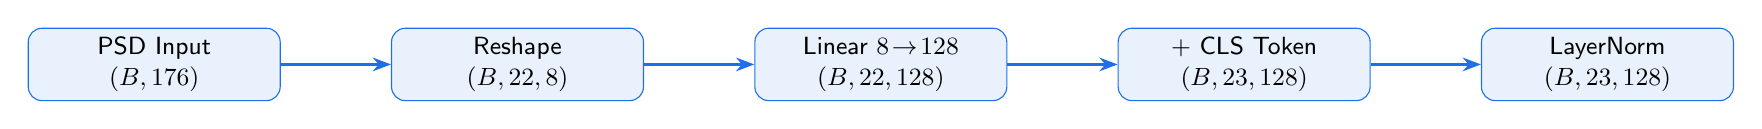
\begin{tikzpicture}[node distance=1.5cm, arr/.style={-Stealth,thick,color=Blue}]
  \node[blk,fill=Blue!10,draw=Blue]       (A)  {PSD Input\\$(B,176)$};
  \node[blk,fill=Blue!10,draw=Blue,right=1.4cm of A] (B)  {Reshape\\$(B,22,8)$};
  \node[blk,fill=Blue!10,draw=Blue,right=1.4cm of B] (C)  {Linear $8\!\to\!128$\\$(B,22,128)$};
  \node[blk,fill=Blue!10,draw=Blue,right=1.4cm of C] (D)  {+ CLS Token\\$(B,23,128)$};
  \node[blk,fill=Blue!10,draw=Blue,right=1.4cm of D] (E)  {LayerNorm\\$(B,23,128)$};
  \draw[arr](A)--(B); \draw[arr](B)--(C); \draw[arr](C)--(D); \draw[arr](D)--(E);
\end{tikzpicture}
\end{center}

% =============================================================================
\subsection{Component 2 — FrequencyAware Positional Encoding}
% =============================================================================

\begin{note}{In Simple Terms}
A Transformer is otherwise \emph{order-blind} — randomly shuffling patches
gives the same result. Positional encoding stamps each patch with its
``address''. This model uses \textbf{two addresses at once}:
a \emph{learned} one (like a name tag) and a
\emph{sinusoidal} one (like a GPS coordinate tied to the actual
radio frequency). They are blended with a learned weight $\alpha$.
\end{note}

\[
  \text{PE} = \sigma(\alpha)\cdot e_{\text{learned}} +
              (1-\sigma(\alpha))\cdot e_{\text{sin}},
  \quad
  e_{\text{sin}}(p,2i) = \sin\!\!\left(\frac{p}{10000^{2i/d}}\right)
\]

\subsubsection{Flowchart}

\begin{center}
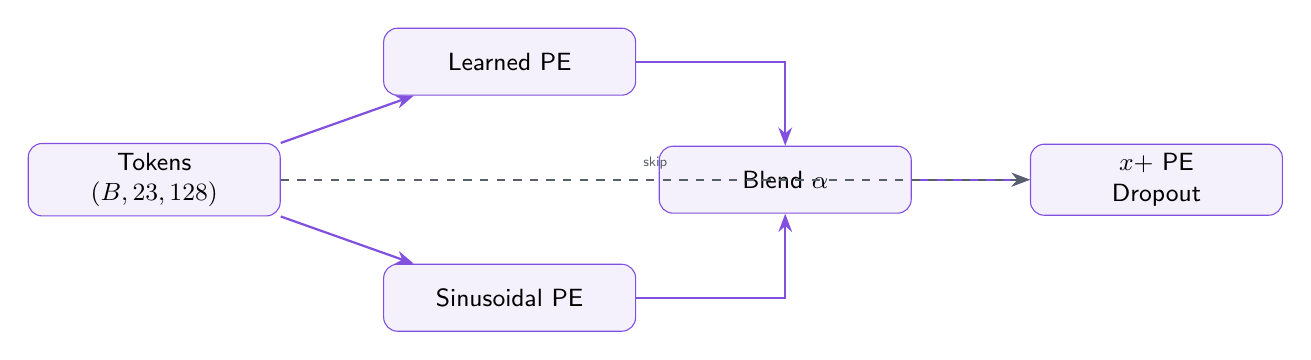
\begin{tikzpicture}[arr/.style={-Stealth,thick,color=Purple}]
  \node[blk,fill=Purple!8,draw=Purple] (A) {Tokens\\$(B,23,128)$};
  \node[blk,fill=Purple!8,draw=Purple, above right=0.6cm and 1.3cm of A] (L) {Learned PE};
  \node[blk,fill=Purple!8,draw=Purple, below right=0.6cm and 1.3cm of A] (S) {Sinusoidal PE};
  \node[blk,fill=Purple!8,draw=Purple, right=4.8cm of A] (B) {Blend $\alpha$};
  \node[blk,fill=Purple!8,draw=Purple, right=1.5cm of B] (C) {$x +$ PE \\ Dropout};
  \draw[arr](A.north east)--(L); \draw[arr](A.south east)--(S);
  \draw[arr](L)-|(B); \draw[arr](S)-|(B);
  \draw[arr](B)--(C);
  \draw[arr,dashed,color=Gray](A.east)--node[above,font=\tiny\sffamily\color{Gray}]{skip} (C.west);
\end{tikzpicture}
\end{center}

% =============================================================================
\subsection{Component 3 — Spectrum Transformer Encoder}
% =============================================================================

\begin{note}{In Simple Terms}
This is the model's \textbf{brain}. It is a stack of 4 identical
``attention'' blocks. In each block, every spectral patch asks:
\emph{``Which other patches are related to me?''} — like finding
which frequency bins correlate (e.g.\ a signal and its sidebands).
\textbf{Pre-LN} (LayerNorm applied \emph{before} attention) keeps
training stable and avoids gradient explosions.
\end{note}

\begin{center}
\renewcommand{\arraystretch}{1.2}
\begin{tabular}{ll}
\toprule
\textbf{Parameter} & \textbf{Value} \\
\midrule
Embedding dimension $d$ & 128 \\
Attention heads         & 4 (each dim = 32) \\
Encoder layers          & 4 \\
Feed-forward hidden dim & 512 \\
Dropout                 & 0.10 \\
Normalisation           & Pre-LN (\texttt{norm\_first=True}) \\
Activation              & GELU \\
Parameters              & $\approx$400 K \\
\bottomrule
\end{tabular}
\end{center}

\medskip\noindent
\textbf{Self-attention core equation:}
\[
  \text{Attention}(Q,K,V) = \text{softmax}\!\left(\frac{QK^\top}{\sqrt{d_k}}\right)V
\]

\subsubsection{Flowchart — One Encoder Layer (×4)}

\begin{center}
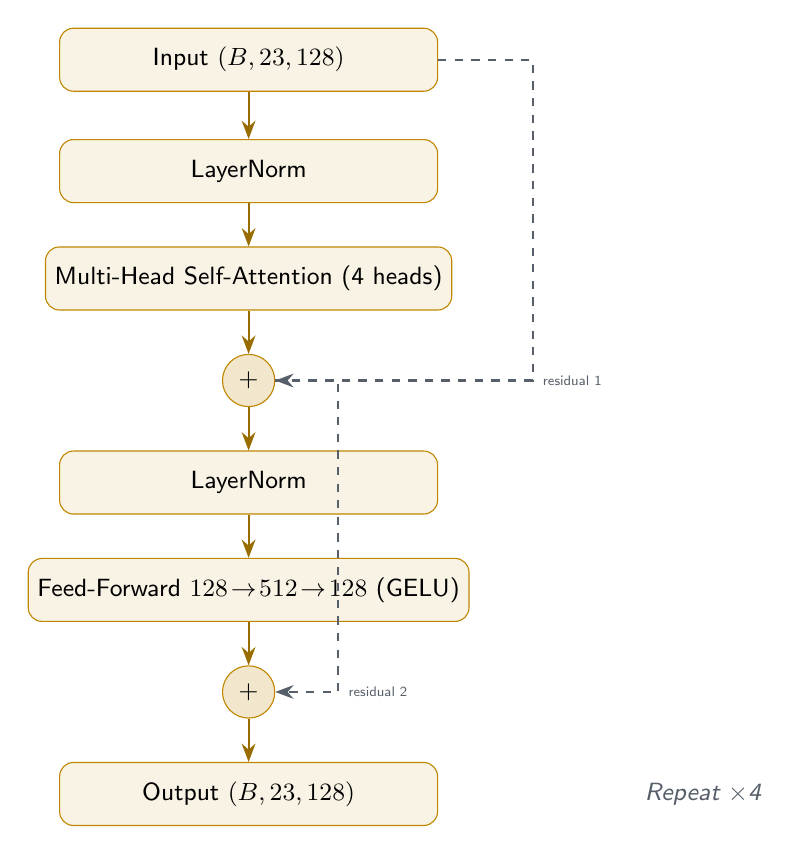
\begin{tikzpicture}[
  node distance=0.7cm,
  blk/.style={draw=Gold,rounded corners=5pt,fill=Gold!10,
              minimum width=4.8cm,minimum height=0.8cm,
              align=center,font=\small\sffamily},
  add/.style={draw=Gold,circle,fill=Gold!20,minimum size=0.6cm,
              font=\small\bfseries},
  arr/.style={-Stealth,thick,color=Gold!80!black},
  res/.style={-Stealth,thick,color=Gray,dashed}
]
  \node[blk]                 (In)   {Input $(B,23,128)$};
  \node[blk,below=0.6cm of In]  (LN1)  {LayerNorm};
  \node[blk,below=0.55cm of LN1](MHSA) {Multi-Head Self-Attention (4 heads)};
  \node[add,below=0.55cm of MHSA](A1)  {$+$};
  \node[blk,below=0.55cm of A1] (LN2)  {LayerNorm};
  \node[blk,below=0.55cm of LN2](FFN)  {Feed-Forward $128\!\to\!512\!\to\!128$ (GELU)};
  \node[add,below=0.55cm of FFN](A2)   {$+$};
  \node[blk,below=0.55cm of A2] (Out)  {Output $(B,23,128)$};

  \draw[arr](In)--(LN1); \draw[arr](LN1)--(MHSA);
  \draw[arr](MHSA)--(A1); \draw[arr](A1)--(LN2);
  \draw[arr](LN2)--(FFN); \draw[arr](FFN)--(A2);
  \draw[arr](A2)--(Out);
  % residuals
  \draw[res](In.east)  -- ++(1.2,0) |- (A1.east)
    node[midway,right,font=\tiny\sffamily\color{Gray}]{residual 1};
  \draw[res](A1.east)  -- ++(0.8,0) |- (A2.east)
    node[midway,right,font=\tiny\sffamily\color{Gray}]{residual 2};
  \node[right=2.5cm of Out,font=\small\sffamily\color{Gray}]{\textit{Repeat $\times$4}};
\end{tikzpicture}
\end{center}

% =============================================================================
\subsection{Component 4 — Multi-Task Output Heads}
% =============================================================================

\begin{note}{In Simple Terms}
After the Transformer, only the \textbf{[CLS] token} output is used.
Think of it as a \emph{meeting-summary sheet} filled in by the model.
This sheet is handed to \textbf{four specialists}, each a tiny
2-layer network:
\begin{enumerate}[nosep]
  \item \textbf{PU Detector} — Is the channel busy? (0 or 1)
  \item \textbf{Modulation Classifier} — Which of 5 modes? (BPSK/QPSK/8PSK/16QAM/DQPSK)
  \item \textbf{SNR Estimator} — Signal strength in dB? (continuous)
  \item \textbf{Generative Head} — Reconstruct the next 176-bin PSD snapshot
\end{enumerate}
\end{note}

\begin{center}
\renewcommand{\arraystretch}{1.25}
\begin{tabular}{lllll}
\toprule
\textbf{Head} & \textbf{Architecture} & \textbf{Output} & \textbf{Loss} & \textbf{Task} \\
\midrule
PUDetectionHead   & $128\!\to\!64\!\to\!2$   & logits $(B,2)$   & Focal Loss ($\gamma{=}2$)  & Binary: busy/idle \\
ModulationHead    & $128\!\to\!64\!\to\!5$   & logits $(B,5)$   & Cross-Entropy              & 5-class modulation \\
SNRHead           & $128\!\to\!64\!\to\!1$   & scalar $(B,)$    & MSE (dB)                   & Signal strength \\
GenerativeHead    & $128\!\to\!256\!\to\!176$ & PSD $(B,176)$   & MSE                        & Next PSD \\
MSMHead (Ph.\,1)  & $128\!\to\!128\!\to\!8$  & patches $(B,22,8)$ & MSE (masked only)        & Pre-training only \\
\bottomrule
\end{tabular}
\end{center}

\subsubsection{Flowchart}

\begin{center}
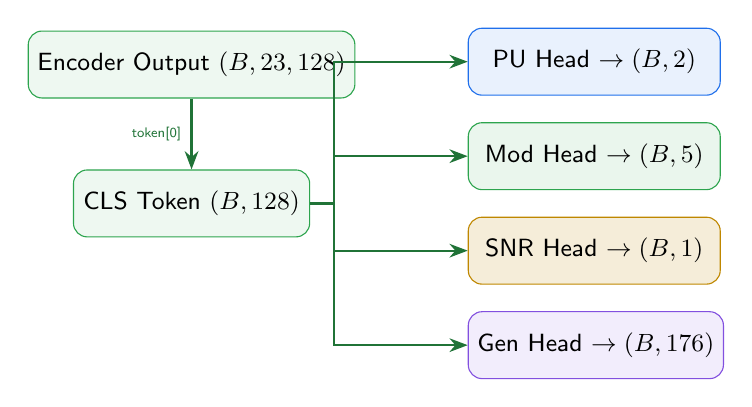
\begin{tikzpicture}[arr/.style={-Stealth,thick,color=Green!70!black}]
  \node[blk,fill=Green!8,draw=Green,minimum width=4cm] (E) {Encoder Output $(B,23,128)$};
  \node[blk,fill=Green!8,draw=Green,minimum width=3cm,below=0.9cm of E] (C)
    {CLS Token $(B,128)$};
  \node[blk,fill=Blue!10,  draw=Blue,  right=2cm of C, yshift= 1.8cm] (H1)
    {PU Head $\to(B,2)$};
  \node[blk,fill=Green!10, draw=Green, right=2cm of C, yshift= 0.6cm] (H2)
    {Mod Head $\to(B,5)$};
  \node[blk,fill=Gold!15,  draw=Gold,  right=2cm of C, yshift=-0.6cm] (H3)
    {SNR Head $\to(B,1)$};
  \node[blk,fill=Purple!10,draw=Purple,right=2cm of C, yshift=-1.8cm] (H4)
    {Gen Head $\to(B,176)$};
  \draw[arr](E)--node[left,font=\tiny\sffamily\color{Gray}]{token[0]}(C);
  \foreach \h in {H1,H2,H3,H4}{ \draw[arr](C.east)--++(0.3,0)|-(\h.west); }
\end{tikzpicture}
\end{center}

% =============================================================================
\subsection{Component 5 — MSMHead (Masked Spectrum Modelling)}
% =============================================================================

\begin{note}{In Simple Terms}
Only active in \textbf{Phase 1}. Borrowed from BERT's masked word prediction:
hide 20\% of the 22 spectral patches (zero them out) and train the model
to \emph{reconstruct} the hidden values. No labels needed — the model
learns spectrum physics from raw, unlabelled data.
\end{note}

\noindent\textbf{Masking rule:} $\;\tilde{x}_i = 0$ if patch $i$ is masked,
$\tilde{x}_i = x_i$ otherwise.

\[
  \mathcal{L}_\text{MSM}
  = \frac{1}{|\mathcal{M}|\cdot 8}
    \sum_{i \in \mathcal{M}} \|\hat{x}_i - x_i\|^2
  \quad (\mathcal{M} = \text{masked patch indices},\; 20\%\text{ of } 22)
\]

\subsubsection{Flowchart}

\begin{center}
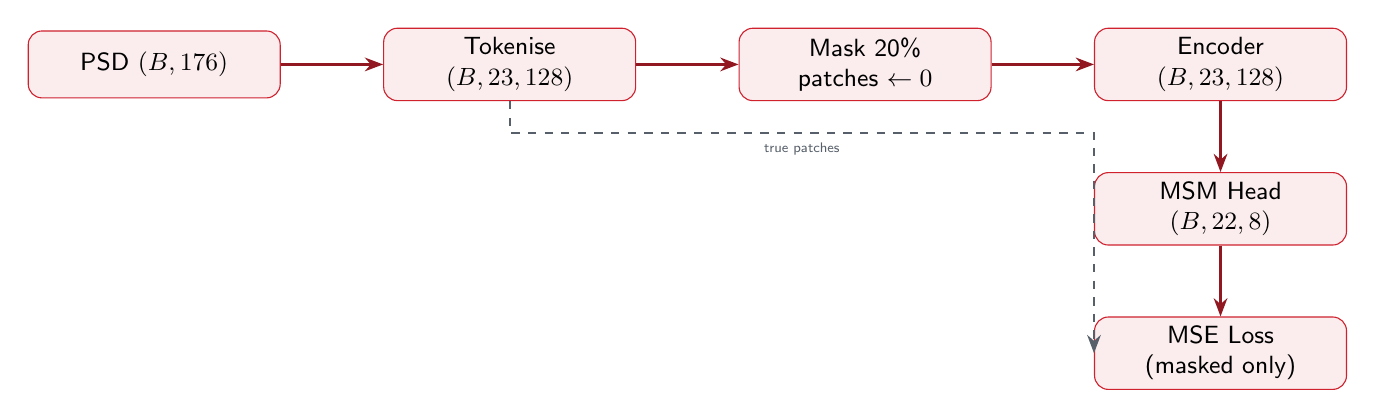
\begin{tikzpicture}[arr/.style={-Stealth,thick,color=Red!70!black}]
  \node[blk,fill=Red!8,draw=Red] (A) {PSD $(B,176)$};
  \node[blk,fill=Red!8,draw=Red,right=1.3cm of A] (B) {Tokenise\\$(B,23,128)$};
  \node[blk,fill=Red!8,draw=Red,right=1.3cm of B] (C) {Mask 20\%\\patches $\leftarrow 0$};
  \node[blk,fill=Red!8,draw=Red,right=1.3cm of C] (D) {Encoder\\$(B,23,128)$};
  \node[blk,fill=Red!8,draw=Red,below=0.9cm of D]  (E) {MSM Head\\$(B,22,8)$};
  \node[blk,fill=Red!8,draw=Red,below=0.9cm of E]  (F) {MSE Loss\\(masked only)};
  \draw[arr](A)--(B); \draw[arr](B)--(C); \draw[arr](C)--(D);
  \draw[arr](D)--(E); \draw[arr](E)--(F);
  \draw[-Stealth,thick,dashed,color=Gray](B.south)--+(0,-0.4)-|(F.west)
    node[near start,below,font=\tiny\sffamily\color{Gray}]{true patches};
\end{tikzpicture}
\end{center}

% =============================================================================
\section{End-to-End Training Pipeline}
% =============================================================================

\begin{center}
\begin{tikzpicture}[
  phase/.style={draw, rounded corners=6pt, align=center,
                minimum width=13cm, minimum height=1cm, font=\small\sffamily},
  step/.style={draw, rounded corners=4pt, align=center,
               minimum width=2.8cm, minimum height=0.8cm, font=\small\sffamily},
  arr/.style={-Stealth, very thick}
]
% ── Row 0: Data
\node[phase, fill=Blue!10, draw=Blue] (D)
  {\textbf{SDR Data:} USRP + GNURadio $\to$ Welch PSD $\to$ 176 bins $\to$
   \texttt{.pth} files (BPSK / QPSK / 16QAM / 8PSK / DQPSK)};

% ── Row 1: Phase 1
\node[phase, fill=Purple!8, draw=Purple, below=0.6cm of D] (P1)
  {\textbf{Phase 1 — Masked Spectrum Modelling (self-supervised, no labels)}};
  
\node[step, fill=Purple!6, draw=Purple, below left=0.6cm and -2.2cm of P1] (p1a)
  {Mask 20\%\\patches};
\node[step, fill=Purple!6, draw=Purple, right=0.3cm of p1a] (p1b) {PatchEmbed\\+ PosEnc};
\node[step, fill=Purple!6, draw=Purple, right=0.3cm of p1b] (p1c) {4-layer\\Transformer};
\node[step, fill=Purple!6, draw=Purple, right=0.3cm of p1c] (p1d) {MSM Head\\MSE Loss};

\draw[arr, color=Purple] (p1a) -- (p1b); 
\draw[arr, color=Purple] (p1b) -- (p1c);
\draw[arr, color=Purple] (p1c) -- (p1d);

% ── Row 2: Phase 2
\node[phase, fill=Green!8, draw=Green, below=1.0cm of p1a, xshift=3.8cm] (P2)
  {\textbf{Phase 2 — Supervised Fine-Tuning (labelled, 5 modulation classes)}};
  
\node[step, fill=Green!6, draw=Green, below left=0.6cm and -2.2cm of P2] (p2a) {Load Ph.1\\weights};
\node[step, fill=Green!6, draw=Green, right=0.3cm of p2a] (p2b) {PatchEmbed\\+ PosEnc};
\node[step, fill=Green!6, draw=Green, right=0.3cm of p2b] (p2c) {4-layer\\Transformer};
\node[step, fill=Green!6, draw=Green, right=0.3cm of p2c] (p2d) {PU+Mod+SNR\\Heads};

\draw[arr, color=Green] (p2a) -- (p2b); 
\draw[arr, color=Green] (p2b) -- (p2c);
\draw[arr, color=Green] (p2c) -- (p2d);

% ── Row 3: Phase 3
\node[phase, fill=Gold!10, draw=Gold, below=1.0cm of p2a, xshift=3.8cm] (P3)
  {\textbf{Phase 3 — Generative Training (predict next PSD snapshot)}};
  
\node[step, fill=Gold!8, draw=Gold, below left=0.6cm and -2.2cm of P3] (p3a) {Load Ph.2\\weights};
\node[step, fill=Gold!8, draw=Gold, right=0.3cm of p3a] (p3b) {Sequence\\$(B,L,176)$};
\node[step, fill=Gold!8, draw=Gold, right=0.3cm of p3b] (p3c) {Transformer\\(shared)};
\node[step, fill=Gold!8, draw=Gold, right=0.3cm of p3c] (p3d) {Gen Head\\MSE Loss};

\draw[arr, color=Gold] (p3a) -- (p3b); 
\draw[arr, color=Gold] (p3b) -- (p3c);
\draw[arr, color=Gold] (p3c) -- (p3d);

% ── phase links
\draw[arr, color=Blue, very thick] (D.south) -- (P1.north);

% Route phase 1 to phase 2 taking care not to go over the steps
\draw[arr, color=Purple, very thick] (p1d.east) -- ++(0.5,0) |- (P2.east) 
  node[pos=0.25, right, text=Gray, font=\tiny\sffamily] {save ckpt};

% Route phase 2 to phase 3
\draw[arr, color=Green, very thick] (p2d.east) -- ++(0.5,0) |- (P3.east)
  node[pos=0.25, right, text=Gray, font=\tiny\sffamily] {save ckpt};

\end{tikzpicture}
\end{center}

% =============================================================================
\section{Loss Functions}
% =============================================================================

\begin{center}
\renewcommand{\arraystretch}{1.3}
\begin{tabular}{lll}
\toprule
\textbf{Task} & \textbf{Loss} & \textbf{Why chosen} \\
\midrule
PU Detection  & Focal Loss \; $-\alpha(1-p_t)^\gamma \log p_t$, $\gamma=2$
              & Down-weights easy examples; handles rare PU=1 samples \\
Modulation    & Cross-Entropy                 & Standard for multi-class classification \\
SNR           & Mean Squared Error (dB)       & Continuous regression \\
Generative    & Mean Squared Error (per bin)  & Reconstruct next PSD vector \\
MSM (Ph.\,1)  & MSE on masked patches only    & Only penalise the hidden positions \\
\midrule
\multicolumn{3}{l}{\textbf{Combined loss (Phase 2):} $\mathcal{L} = 1.0\,\mathcal{L}_\text{PU} + 0.5\,\mathcal{L}_\text{mod} + 0.3\,\mathcal{L}_\text{SNR}$} \\
\bottomrule
\end{tabular}
\end{center}

% =============================================================================
\section{Design Decisions — Why These Choices?}
% =============================================================================

\begin{center}
\renewcommand{\arraystretch}{1.3}
\begin{tabularx}{\textwidth}{l X X}
\toprule
\textbf{Choice} & \textbf{Reason} & \textbf{Alternative rejected} \\
\midrule
Transformer over CNN
  & Self-attention finds \emph{long-range} bin correlations (harmonics,
    wideband interference) that CNN kernels miss.
  & 1-D CNN (DeepSig-style) \\
Patch tokenisation
  & Cuts sequence length $176\to22$ — attention cost drops
    by $64\times$ ($O(22^2)$ vs $O(176^2)$).
  & Point-by-point tokens \\
3-phase training
  & Phase 1 pre-training on unlabelled data is ``free'' and
    boosts representations before labelled fine-tuning.
  & Train supervised only \\
Multi-task heads
  & PU detection + modulation share a backbone → mutual benefit.
  & Separate models per task \\
Focal Loss for PU
  & Real deployments have very few PU=1 events.
    Focal loss prevents always predicting ``idle''.
  & Standard cross-entropy \\
Pre-LN normalisation
  & Far more stable gradients at the start of training.
  & Post-LN (original Transformer) \\
\bottomrule
\end{tabularx}
\end{center}

% =============================================================================
\section{Parameter Summary}
% =============================================================================

\begin{center}
\renewcommand{\arraystretch}{1.25}
\begin{tabular}{lrl}
\toprule
\textbf{Module} & \textbf{Parameters} & \textbf{Note} \\
\midrule
PatchEmbedding               & $\approx$2 K   & Linear $8\!\times\!128$ + CLS token \\
FreqAware PositionalEncoding & $\approx$3 K   & Embedding table + scalar $\alpha$ \\
Transformer Encoder (4 layers) & $\approx$400 K & MHSA + FFN per layer \\
PUDetectionHead              & $\approx$9 K   & $128\!\to\!64\!\to\!2$ \\
ModulationHead               & $\approx$9 K   & $128\!\to\!64\!\to\!5$ \\
SNRHead                      & $\approx$8 K   & $128\!\to\!64\!\to\!1$ \\
GenerativeHead               & $\approx$78 K  & $128\!\to\!256\!\to\!176$ \\
MSMHead                      & $\approx$17 K  & $128\!\to\!128\!\to\!8$ \\
\midrule
\textbf{Total}               & $\approx$\textbf{1 M} & Edge-deployable \\
\bottomrule
\end{tabular}
\end{center}

% =============================================================================
\section{Glossary}
% =============================================================================

\begin{center}
\renewcommand{\arraystretch}{1.25}
\begin{tabular}{ll}
\toprule
\textbf{Term} & \textbf{Meaning} \\
\midrule
PSD      & Power Spectral Density — energy vs frequency in dB \\
SDR      & Software-Defined Radio (here: a USRP B210) \\
GNURadio & Open-source toolkit for capturing SDR data \\
PU       & Primary User — licensed spectrum holder \\
SNR      & Signal-to-Noise Ratio in dB \\
CLS      & Classification token — global summary of all patches \\
MSM      & Masked Spectrum Modelling — Phase 1 self-supervised task \\
SFT      & Supervised Fine-Tuning — Phase 2 labelled training \\
BPSK     & Binary PSK — 1 bit/symbol, narrowest spectrum \\
QPSK     & Quadrature PSK — 2 bits/symbol \\
8PSK     & 8-level PSK — 3 bits/symbol \\
16QAM    & 16-level QAM — 4 bits/symbol, wider bandwidth \\
DQPSK    & Differential QPSK — robust to phase ambiguity (added Phase 2) \\
Pre-LN   & LayerNorm \emph{before} attention (more stable than post-LN) \\
GELU     & Activation function used in the feed-forward layers \\
\bottomrule
\end{tabular}
\end{center}

% ── Footer ────────────────────────────────────────────────────────────────────
\vfill
\begin{center}\small\color{Gray}
  Spectrum-SLM Technical Reference \textbullet{}
  Anjani, Ashish Joshi, Mayank \textbullet{}
  Guide: Dr.~Abhinandan S.P. \textbullet{} April 2026
\end{center}

\end{document}
